\documentclass[aspectratio=169,11pt]{beamer}

\usepackage[utf8]{inputenc}
\usepackage[T1]{fontenc}
\usepackage{lmodern}
\usepackage{booktabs}
\usepackage{tabularx}
\usepackage{graphicx}

\graphicspath{{../outputs/stationary/hong_nz14_DRSGobel/plots_moll/}}

\definecolor{Ink}{HTML}{1F2933}
\definecolor{Muted}{HTML}{52606D}
\definecolor{Accent}{HTML}{006D77}
\definecolor{Warn}{HTML}{B45309}
\definecolor{Good}{HTML}{0F766E}
\definecolor{Bad}{HTML}{B91C1C}
\definecolor{Soft}{HTML}{F3F4F6}

\setbeamercolor{normal text}{fg=Ink,bg=white}
\setbeamercolor{frametitle}{fg=Ink,bg=white}
\setbeamercolor{title}{fg=Ink}
\setbeamercolor{structure}{fg=Accent}
\setbeamercolor{block title}{fg=white,bg=Accent}
\setbeamercolor{block body}{fg=Ink,bg=Soft}
\setbeamertemplate{navigation symbols}{}
\setbeamertemplate{itemize item}{\color{Accent}$\blacktriangleright$}
\setbeamertemplate{footline}{%
  \leavevmode%
  \hbox{%
    \begin{beamercolorbox}[wd=.78\paperwidth,ht=2.5ex,dp=1.2ex,leftskip=1.5em]{author in head/foot}%
      \scriptsize Informalidad y distribuci\'on de riqueza
    \end{beamercolorbox}%
    \begin{beamercolorbox}[wd=.22\paperwidth,ht=2.5ex,dp=1.2ex,rightskip=1.5em plus1fil]{date in head/foot}%
      \scriptsize \insertframenumber/\inserttotalframenumber
    \end{beamercolorbox}}%
  \vskip0pt%
}

\newcommand{\statusok}{\textcolor{Good}{\textbf{OK}}}
\newcommand{\statuslow}{\textcolor{Warn}{\textbf{Bajo}}}
\newcommand{\statusstruct}{\textcolor{Bad}{\textbf{Estructural}}}

\title{Informalidad y Distribuci\'on de Riqueza}
\subtitle{Modelo de agentes heterog\'eneos con oferta laboral end\'ogena}
\author{John Svante Barraza Ratachi \and Enzo Andr\'es Nevado Mart\'inez}
\institute{Asesor: C\'esar Saturnino Salinas Depaz}
\date{Junio de 2026}

\begin{document}

\begin{frame}[plain]
  \vspace{0.7cm}
  {\huge \textbf{Informalidad y Distribuci\'on de Riqueza}}\\[0.25cm]
  {\Large Modelo de agentes heterog\'eneos con oferta laboral end\'ogena}\\[0.9cm]
  \begin{tabular}{rl}
    \textbf{Autores:} & John Svante Barraza Ratachi \\
                      & Enzo Andr\'es Nevado Mart\'inez \\[0.15cm]
    \textbf{Asesor:} & C\'esar Saturnino Salinas Depaz
  \end{tabular}\\[0.6cm]
  {\large Junio de 2026}
\end{frame}

\begin{frame}{Motivaci\'on y pregunta}
  \begin{columns}[T,onlytextwidth]
    \begin{column}{0.48\textwidth}
      \textbf{Problema}
      \begin{itemize}
        \item Per\'u: alta informalidad laboral (55.7\%) con desigualdad patrimonial elevada.
        \item Evidencia directa de riqueza por hogar es limitada (sin encuesta de riqueza).
        \item La informalidad afecta ingresos, ahorro, cr\'edito y acumulaci\'on.
      \end{itemize}
      \vspace{0.2cm}
      \textbf{Hip\'otesis}
      \begin{itemize}
        \item Trampa de baja acumulaci\'on: hogares con menor riqueza y productividad dependen m\'as del sector informal $\rightarrow$ menor ahorro.
      \end{itemize}
    \end{column}
    \begin{column}{0.48\textwidth}
      \textbf{Pregunta central}
      \begin{itemize}
        \item \textit{¿C\'omo afecta la asignaci\'on de horas entre sector formal e informal a la distribuci\'on de riqueza y consumo?}
      \end{itemize}
      \vspace{0.2cm}
      \textbf{Alcance}
      \begin{itemize}
        \item Margen \textbf{intensivo}: horas, no elecci\'on binaria.
        \item Hogares \textit{ex ante} iguales; \textit{ex post} difieren por riqueza $a$ y productividad $z$.
        \item Objetivo: cuantificar el canal de acumulaci\'on, no explicar todas las causas.
      \end{itemize}
    \end{column}
  \end{columns}
\end{frame}

\begin{frame}{Literatura relacionada}
  \footnotesize
  \begin{columns}[T,onlytextwidth]
    \begin{column}{0.50\textwidth}
      \textbf{Informalidad, ingresos y cr\'edito}
      \begin{itemize}
        \item Engbom et al.\ (2022): salarios informales menores en Brasil.
        \item Gomes et al.\ (2020): transiciones formal--informal como shocks negativos de ingreso.
        \item Granda (2015), Flabbi \& Tejada (2022): menor ahorro y acceso a cr\'edito para informales.
        \item Stiglitz \& Weiss (1992): racionamiento crediticio por informaci\'on asim\'etrica.
      \end{itemize}
      \vspace{0.1cm}
      \textbf{Riqueza y fricciones financieras}
      \begin{itemize}
        \item Buera, Kaboski \& Shin (2011): restricciones crediticias $\rightarrow$ mala asignaci\'on capital--talento.
        \item Albertini, Fairise \& Terriau (2020): informalidad reduce acumulaci\'on de riqueza en ciclo de vida.
      \end{itemize}
    \end{column}
    \begin{column}{0.46\textwidth}
      \textbf{Referencia principal}
      \begin{itemize}
        \item \textbf{Galindo et al.\ (2024, BCRP)}: HACT Per\'u con dos tipos \textbf{ex-ante} (formal/informal fijo). Informalidad reduce riqueza agregada.
        \item \textbf{Este trabajo}: hogares \textit{ex ante} iguales $\rightarrow$ informalidad es resultado \textit{ex post} de decisiones \'optimas.
      \end{itemize}
      \vspace{0.1cm}
      \textbf{Oferta laboral en HA}
      \begin{itemize}
        \item Pijoan-M\'as (2006): ahorro precautorio cae con oferta laboral flexible.
        \item Marcet, Obiols-Homs \& Weil (2007): oferta laboral end\'ogena modifica acumulaci\'on y horas agregadas.
      \end{itemize}
      \vspace{0.1cm}
      \textbf{Paradigmas}
      \begin{itemize}
        \item Estructuralismo (CEPAL/PREALC): heterogeneidad productiva.
        \item Institucional (De Soto, Loayza): barreras burocr\'aticas y costos de formalidad.
      \end{itemize}
    \end{column}
  \end{columns}
\end{frame}

\begin{frame}{Aporte de esta investigaci\'on}
  \small
  \begin{columns}[T,onlytextwidth]
    \begin{column}{0.50\textwidth}
      \textbf{¿Qu\'e extiende respecto a Galindo et al.\ (2024)?}
      \begin{enumerate}
        \item \textbf{Oferta laboral end\'ogena}: los hogares eligen horas; la informalidad no es un tipo fijo ex-ante.
        \item \textbf{Consumo CES + $p_I$ end\'ogeno}: canasta formal/informal con precio de equilibrio.
        \item \textbf{Prima de deuda por productividad}: spread$(z)$ captura racionamiento crediticio diferenciado.
        \item \textbf{Proceso OU}: productividad AR(1) en tiempo continuo, estimado con panel ENAHO 2015--2019.
      \end{enumerate}
    \end{column}
    \begin{column}{0.46\textwidth}
      \textbf{Contribuciones}
      \begin{enumerate}
        \item \textbf{Macroeconom\'ia cuantitativa}: primer HACT con oferta laboral dual y consumo CES calibrado para Per\'u.
        \item \textbf{Canal de acumulaci\'on}: identifica mecanismo informalidad $\rightarrow$ riqueza usando solo datos agregados.
        \item \textbf{Supera barrera de datos}: no requiere microdatos de riqueza por hogar.
      \end{enumerate}
      \vspace{0.15cm}
      \textbf{Novedad metodol\'ogica}
      \begin{itemize}
        \item Hogares \textit{ex ante} iguales; \textit{ex post} la informalidad es resultado end\'ogeno de decisiones \'optimas, no una caracter\'istica prefijada.
      \end{itemize}
    \end{column}
  \end{columns}
\end{frame}

\begin{frame}{Modelo: qu\'e captura}
  \small
  \begin{columns}[T,onlytextwidth]
    \begin{column}{0.50\textwidth}
      \textbf{Hogares}
      \begin{itemize}
        \item Ex ante son iguales: no nacen como formales o informales.
        \item Ex post difieren por riqueza $a$ y productividad idiosincr\'atica $z$.
        \item Eligen consumo formal/informal, horas formales/informales y ahorro o deuda.
      \end{itemize}
    \end{column}
    \begin{column}{0.46\textwidth}
      \textbf{Mercado dual}
      \begin{itemize}
        \item Sector formal y sector informal con tecnolog\'ias distintas.
        \item Barrera reducida de acceso formal $F(z)$, mayor para baja productividad.
        \item Precio informal $p_I$ y tasa de inter\'es se determinan en equilibrio.
      \end{itemize}
    \end{column}
  \end{columns}
  \vspace{0.25cm}
  \begin{block}{Canal econ\'omico}
    Menor productividad $\rightarrow$ m\'as informalidad relativa y m\'as endeudamiento $\rightarrow$ menor acumulaci\'on de riqueza.
  \end{block}
\end{frame}


\begin{frame}{Sorting laboral por productividad}
  \centering
  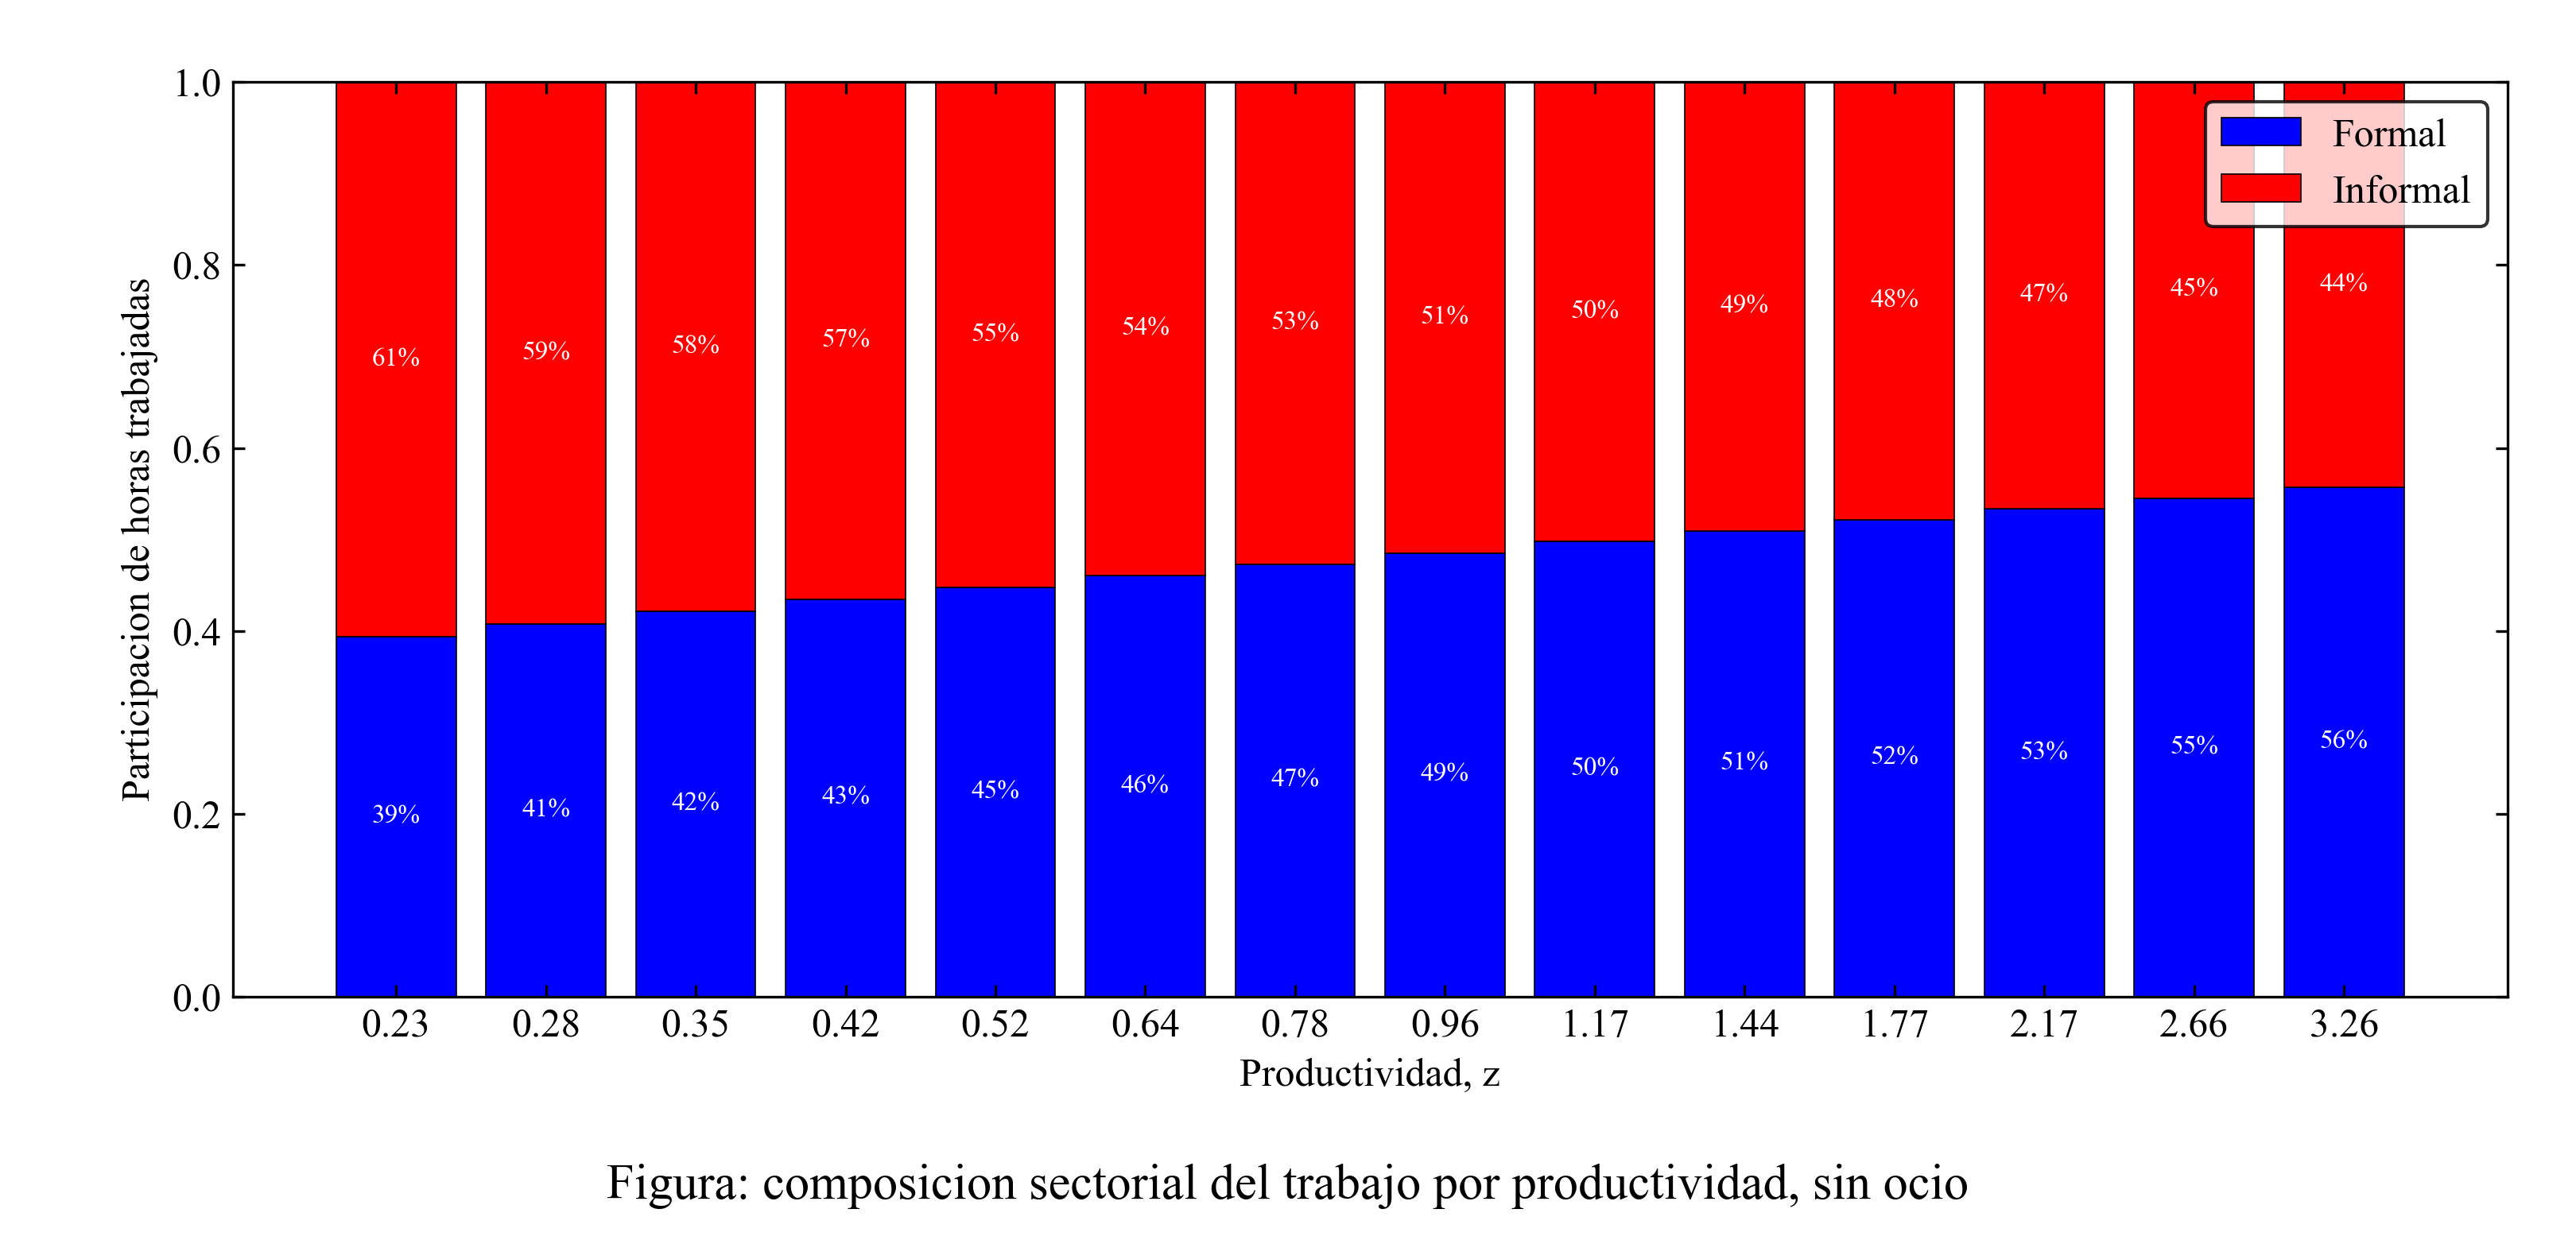
\includegraphics[width=0.94\textwidth,height=0.72\textheight,keepaspectratio]{moll_time_use_by_z_excluding_leisure.png}
  \vspace{0.1cm}

  \small
  La participaci\'on formal aumenta con la productividad $z$; la informalidad domina en estados de baja productividad.
\end{frame}

\begin{frame}{Ahorro y distribuci\'on de riqueza}
  \centering
  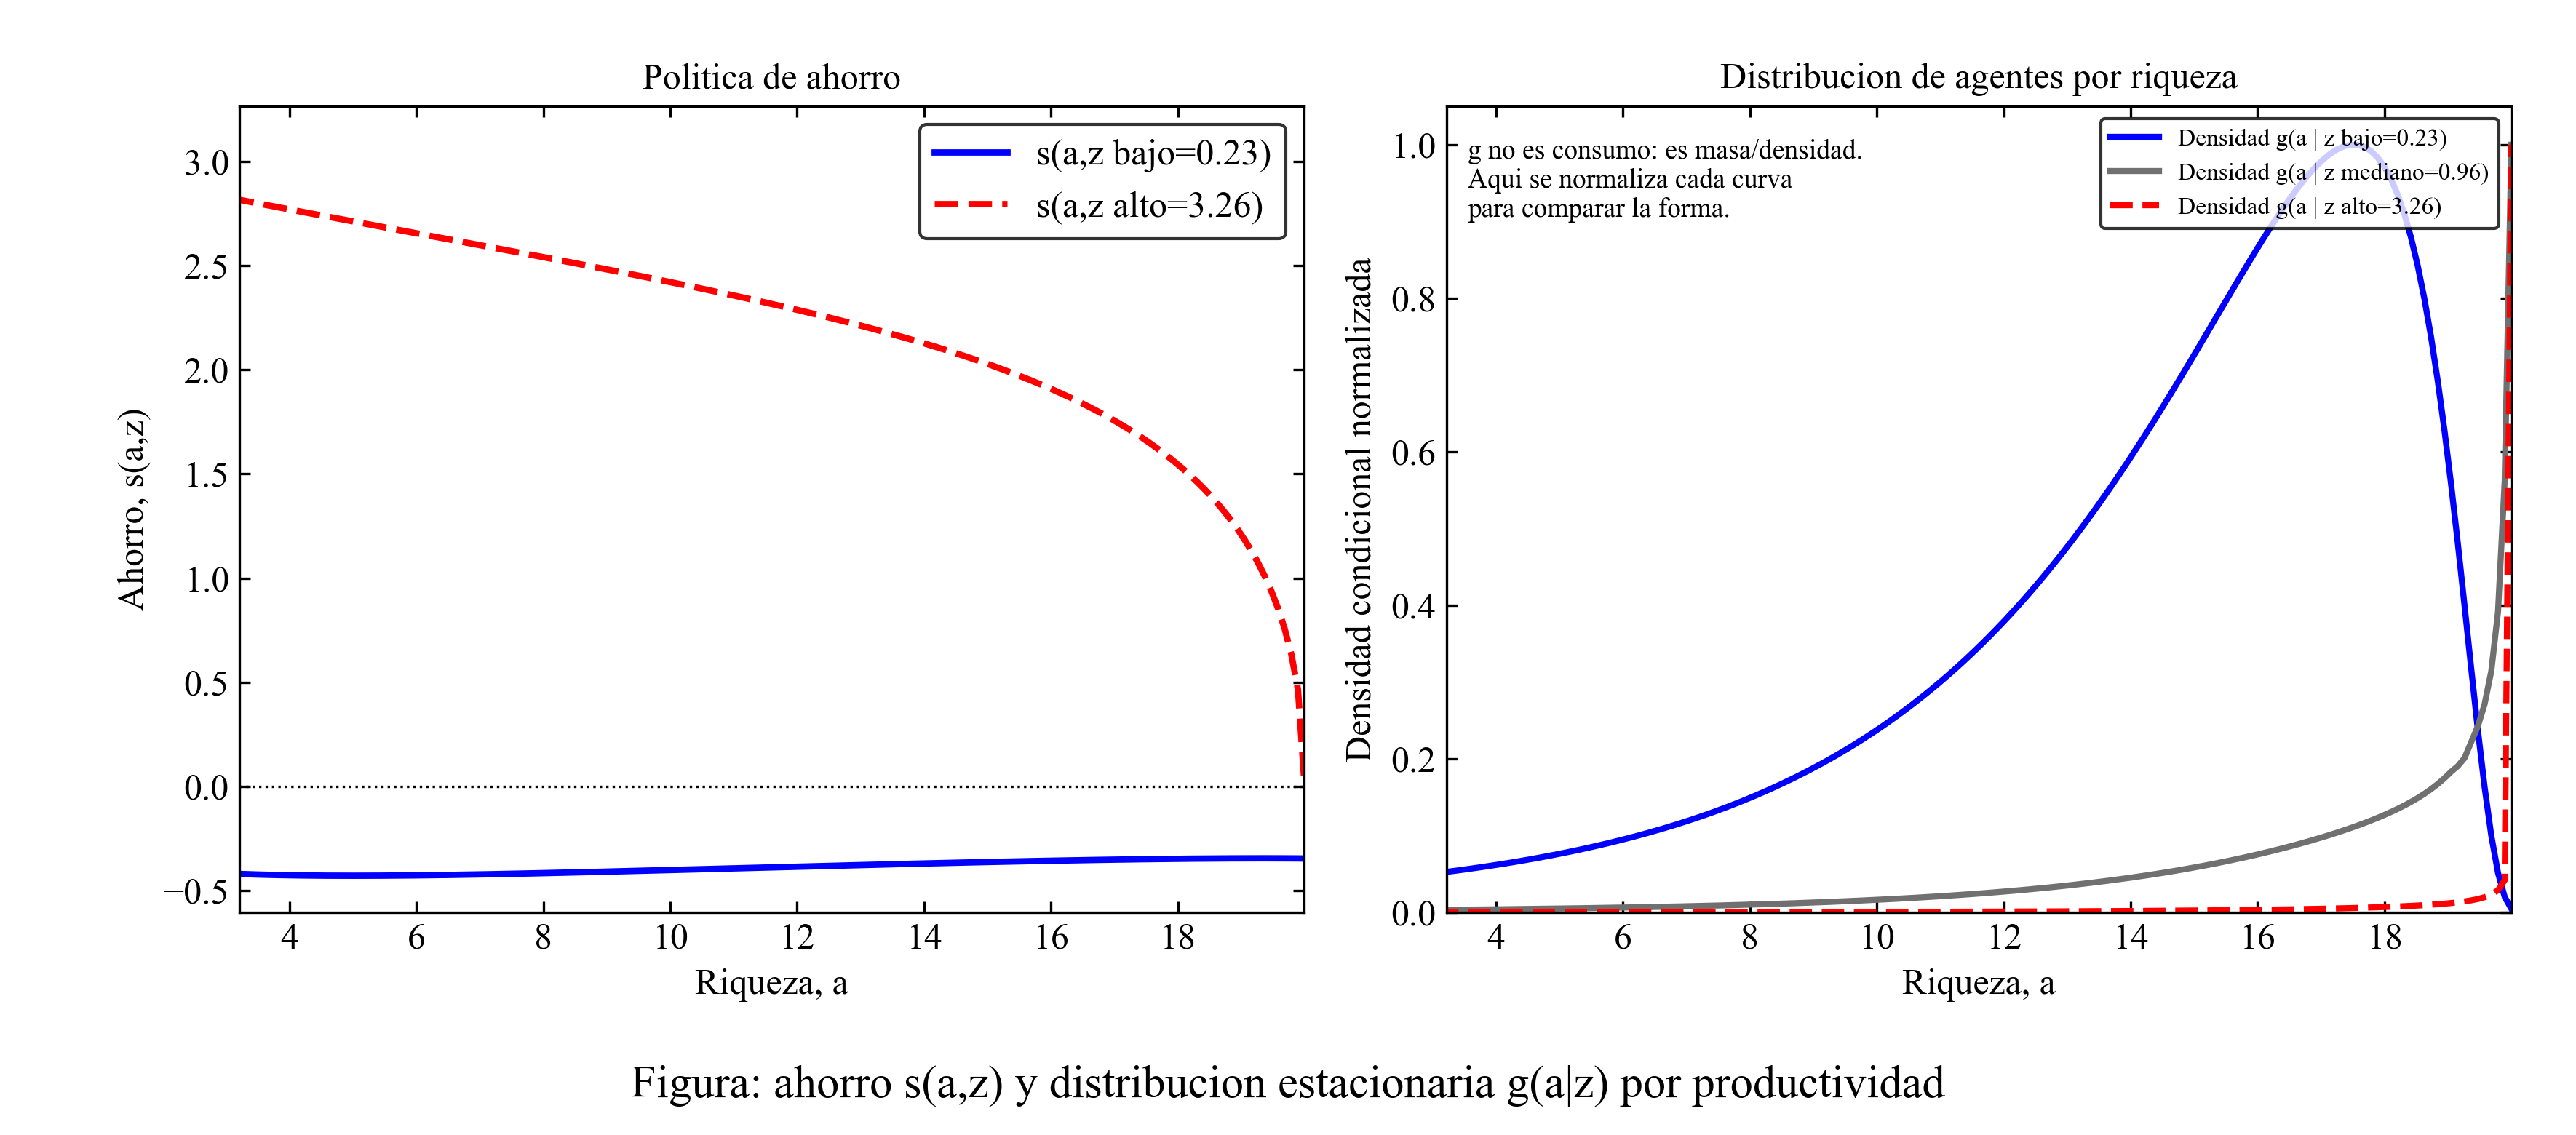
\includegraphics[width=0.94\textwidth,height=0.72\textheight,keepaspectratio]{moll_savings_and_wealth_distribution.png}
  \vspace{0.1cm}

  \small
  Los agentes de baja productividad se concentran en menor riqueza; los de alta productividad acumulan m\'as activos.
\end{frame}

\begin{frame}{Densidad de riqueza por productividad}
  \centering
  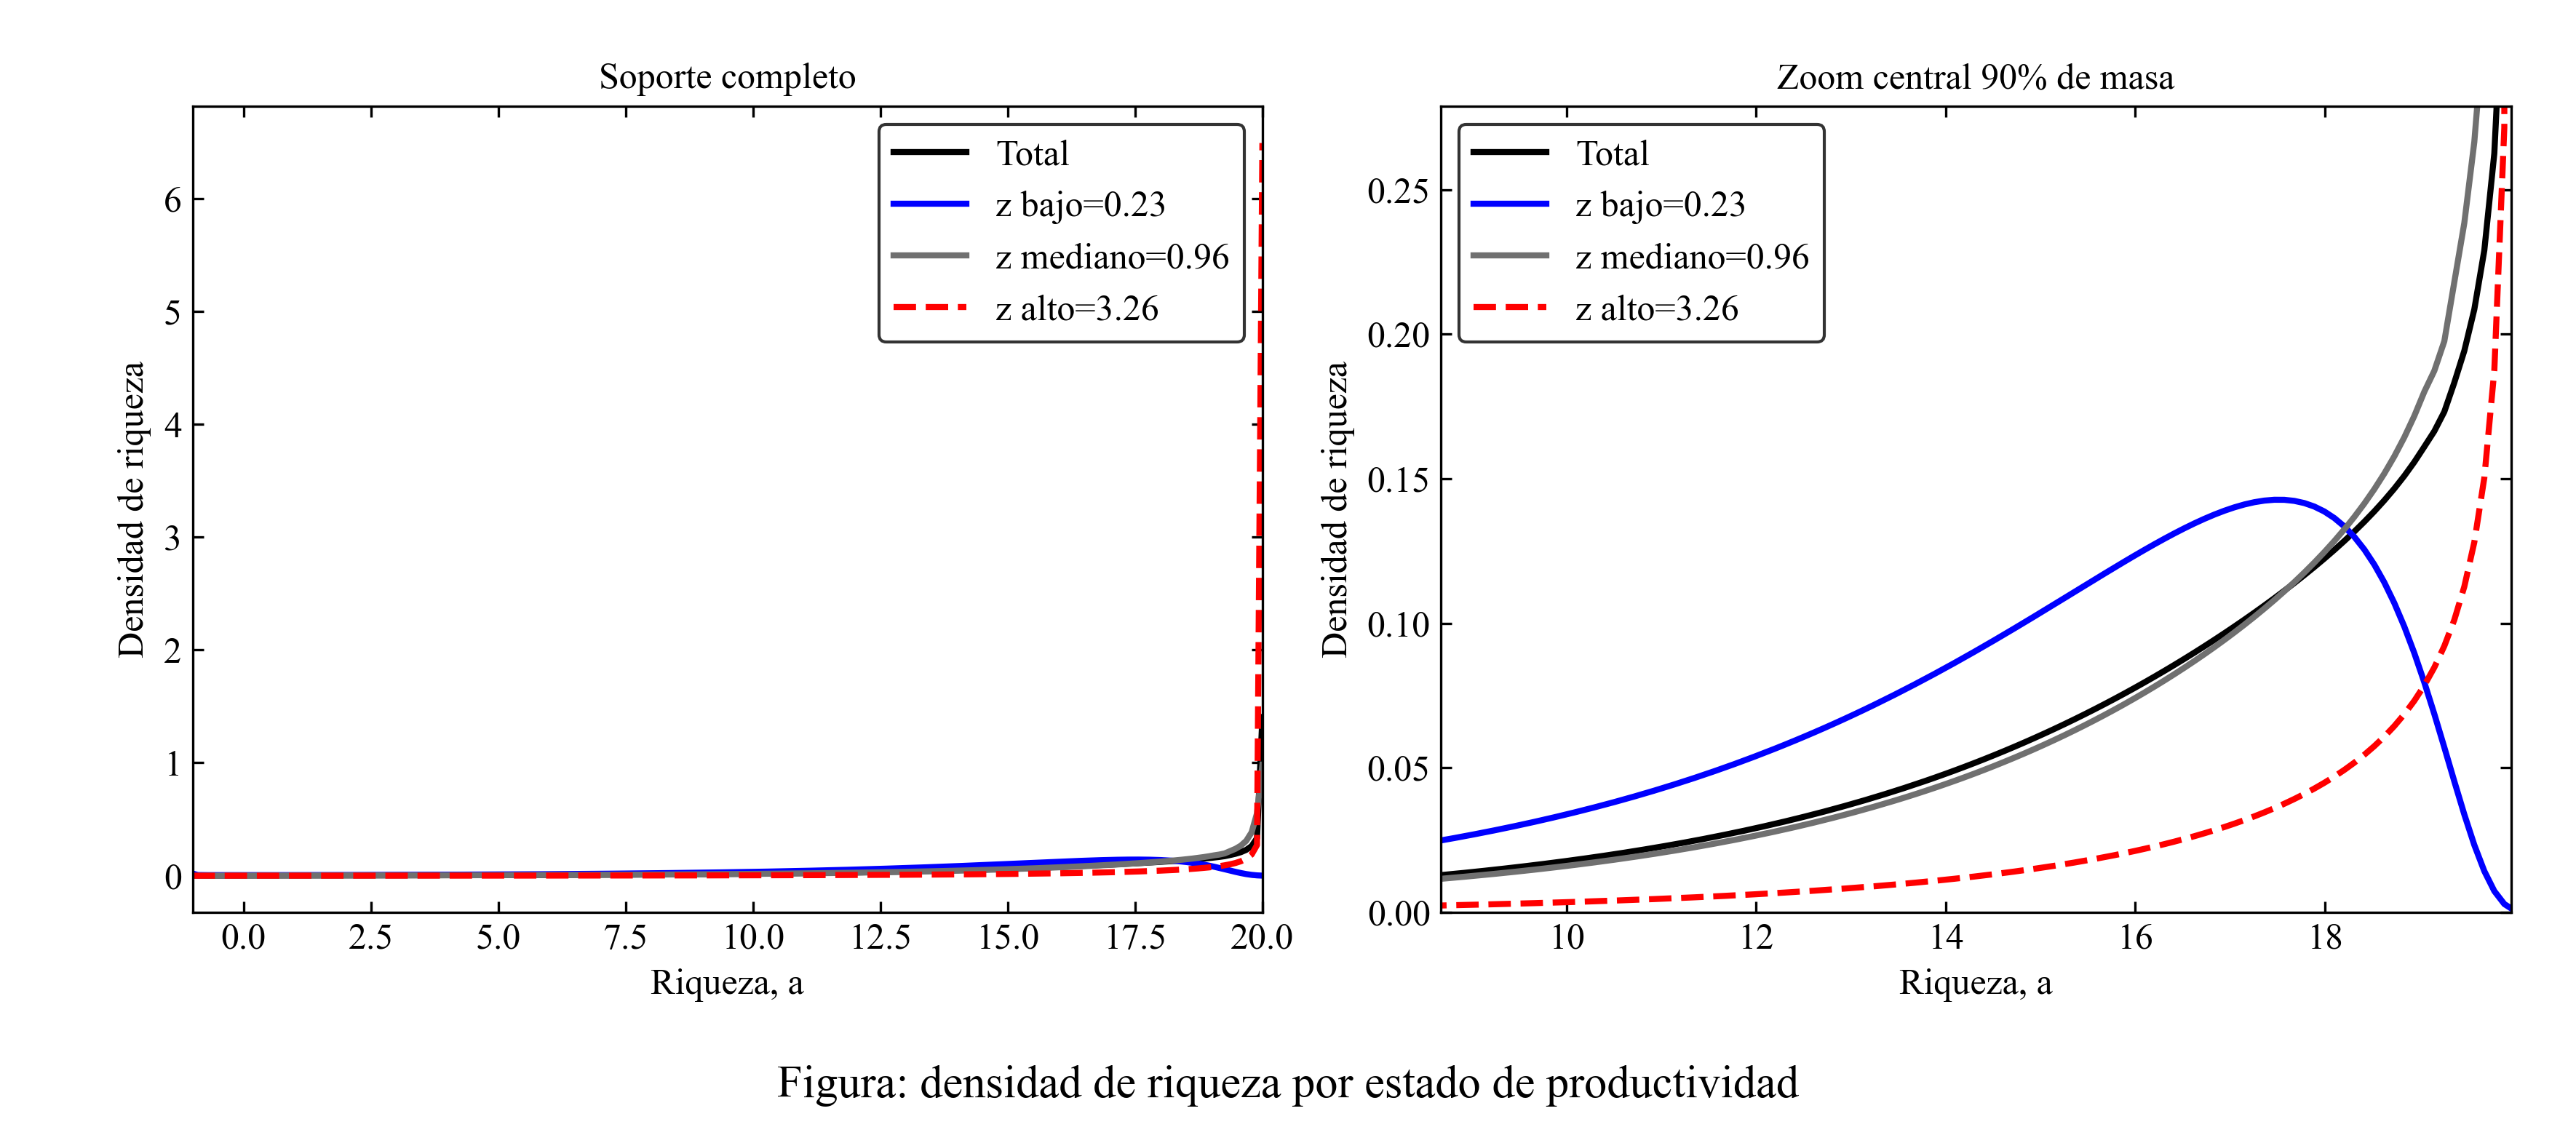
\includegraphics[width=0.94\textwidth,height=0.72\textheight,keepaspectratio]{moll_wealth_density_by_z_low_median_high.png}
  \vspace{0.1cm}

  \small
  La distribuci\'on condicional desplaza masa hacia mayor riqueza cuando aumenta $z$.
\end{frame}

\begin{frame}{Descomposici\'on del ingreso por quintiles}
  \centering
  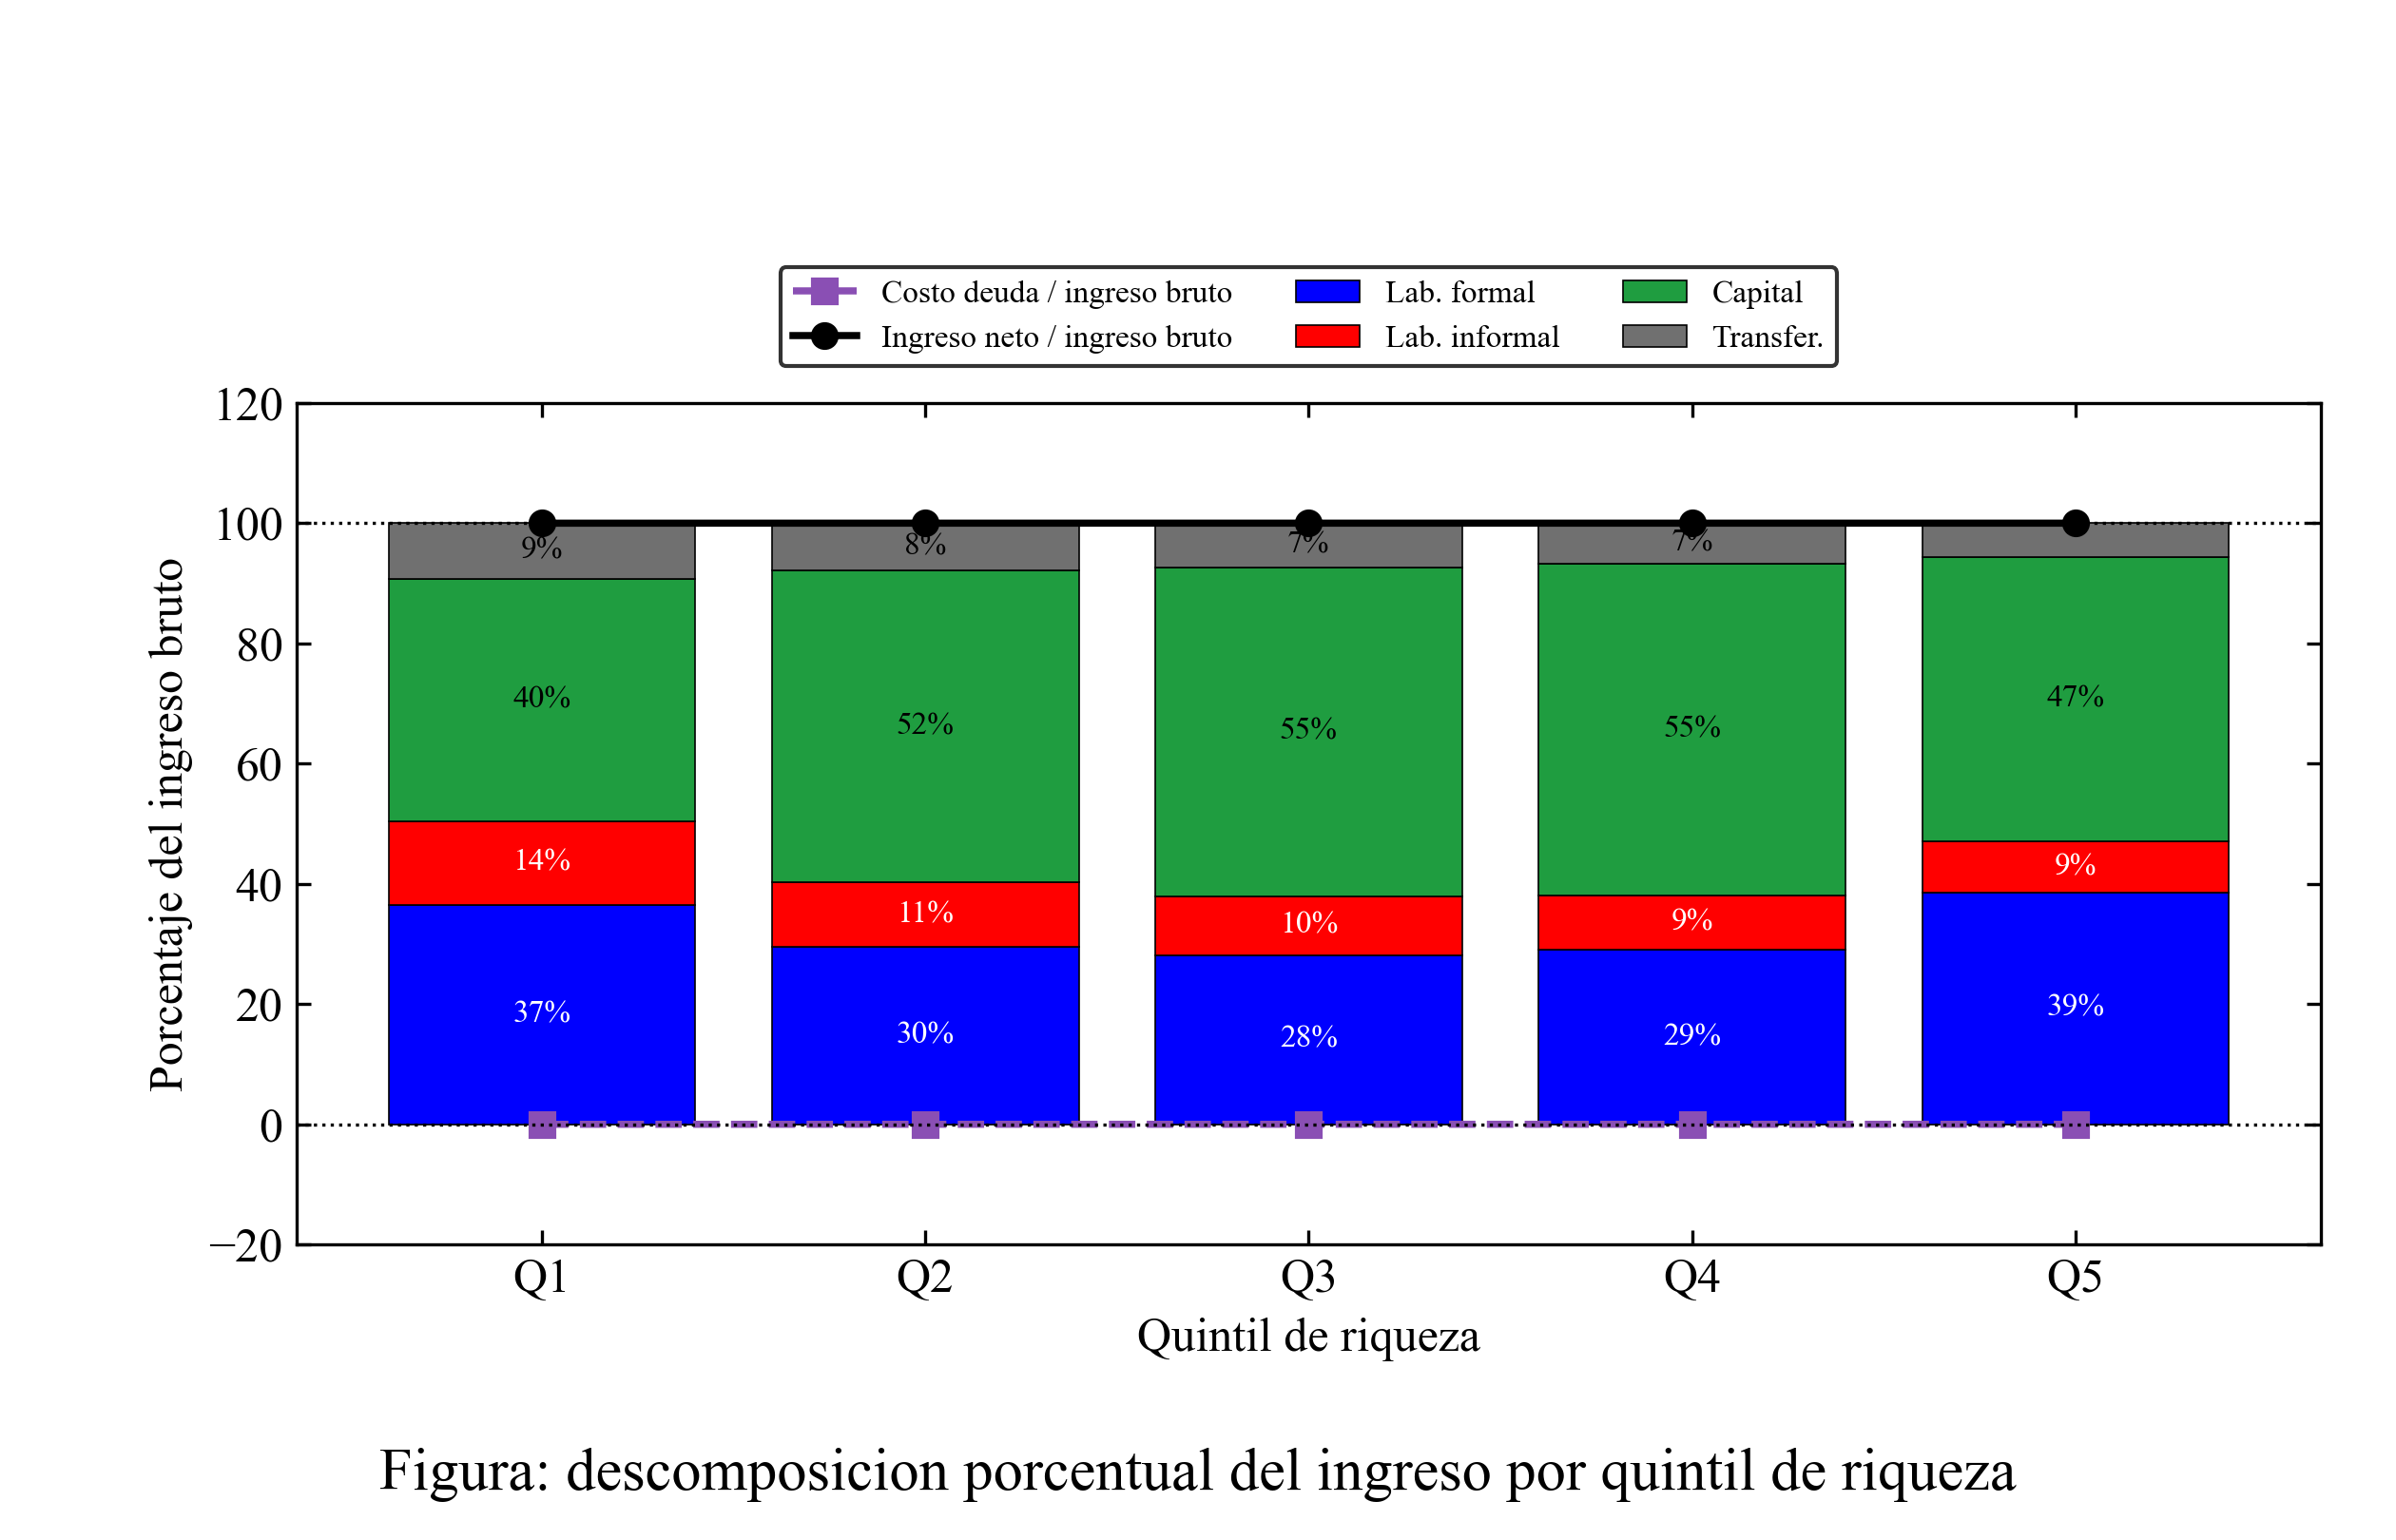
\includegraphics[width=0.94\textwidth,height=0.72\textheight,keepaspectratio]{moll_income_decomposition_percent_by_wealth_quintile.png}
  \vspace{0.1cm}

  \small
  Los quintiles altos dependen relativamente m\'as de ingreso formal y activos; los bajos quedan m\'as expuestos a informalidad y menor acumulaci\'on.
\end{frame}

\begin{frame}{Gasto por formalidad dominante}
  \centering
  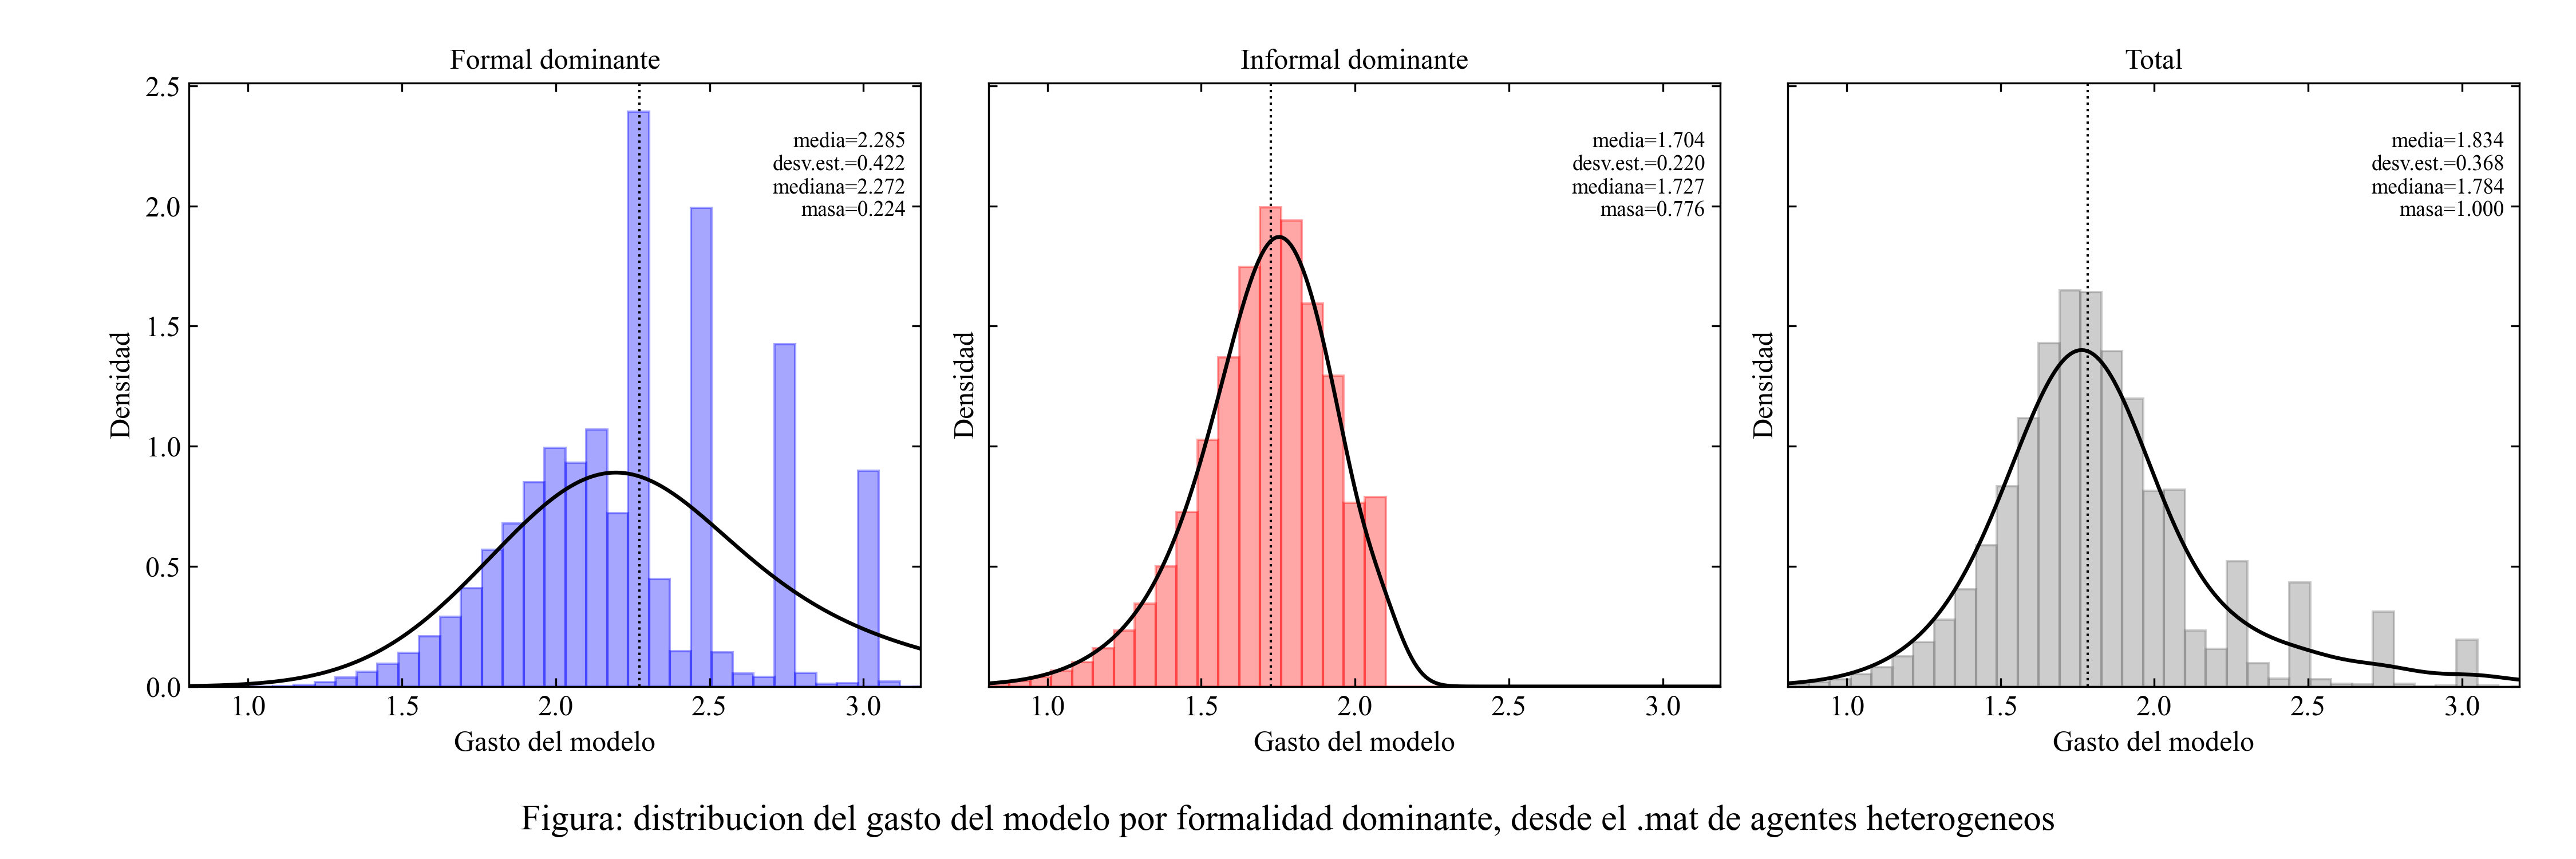
\includegraphics[width=0.94\textwidth,height=0.72\textheight,keepaspectratio]{moll_model_gasto_distribution_by_formality.png}
  \vspace{0.1cm}

  \small
  El modelo predice mayor gasto promedio para hogares formal-dominantes, aunque subestima la brecha observada en datos.
\end{frame}

\begin{frame}{Consumo y componentes de gasto}
  \centering
  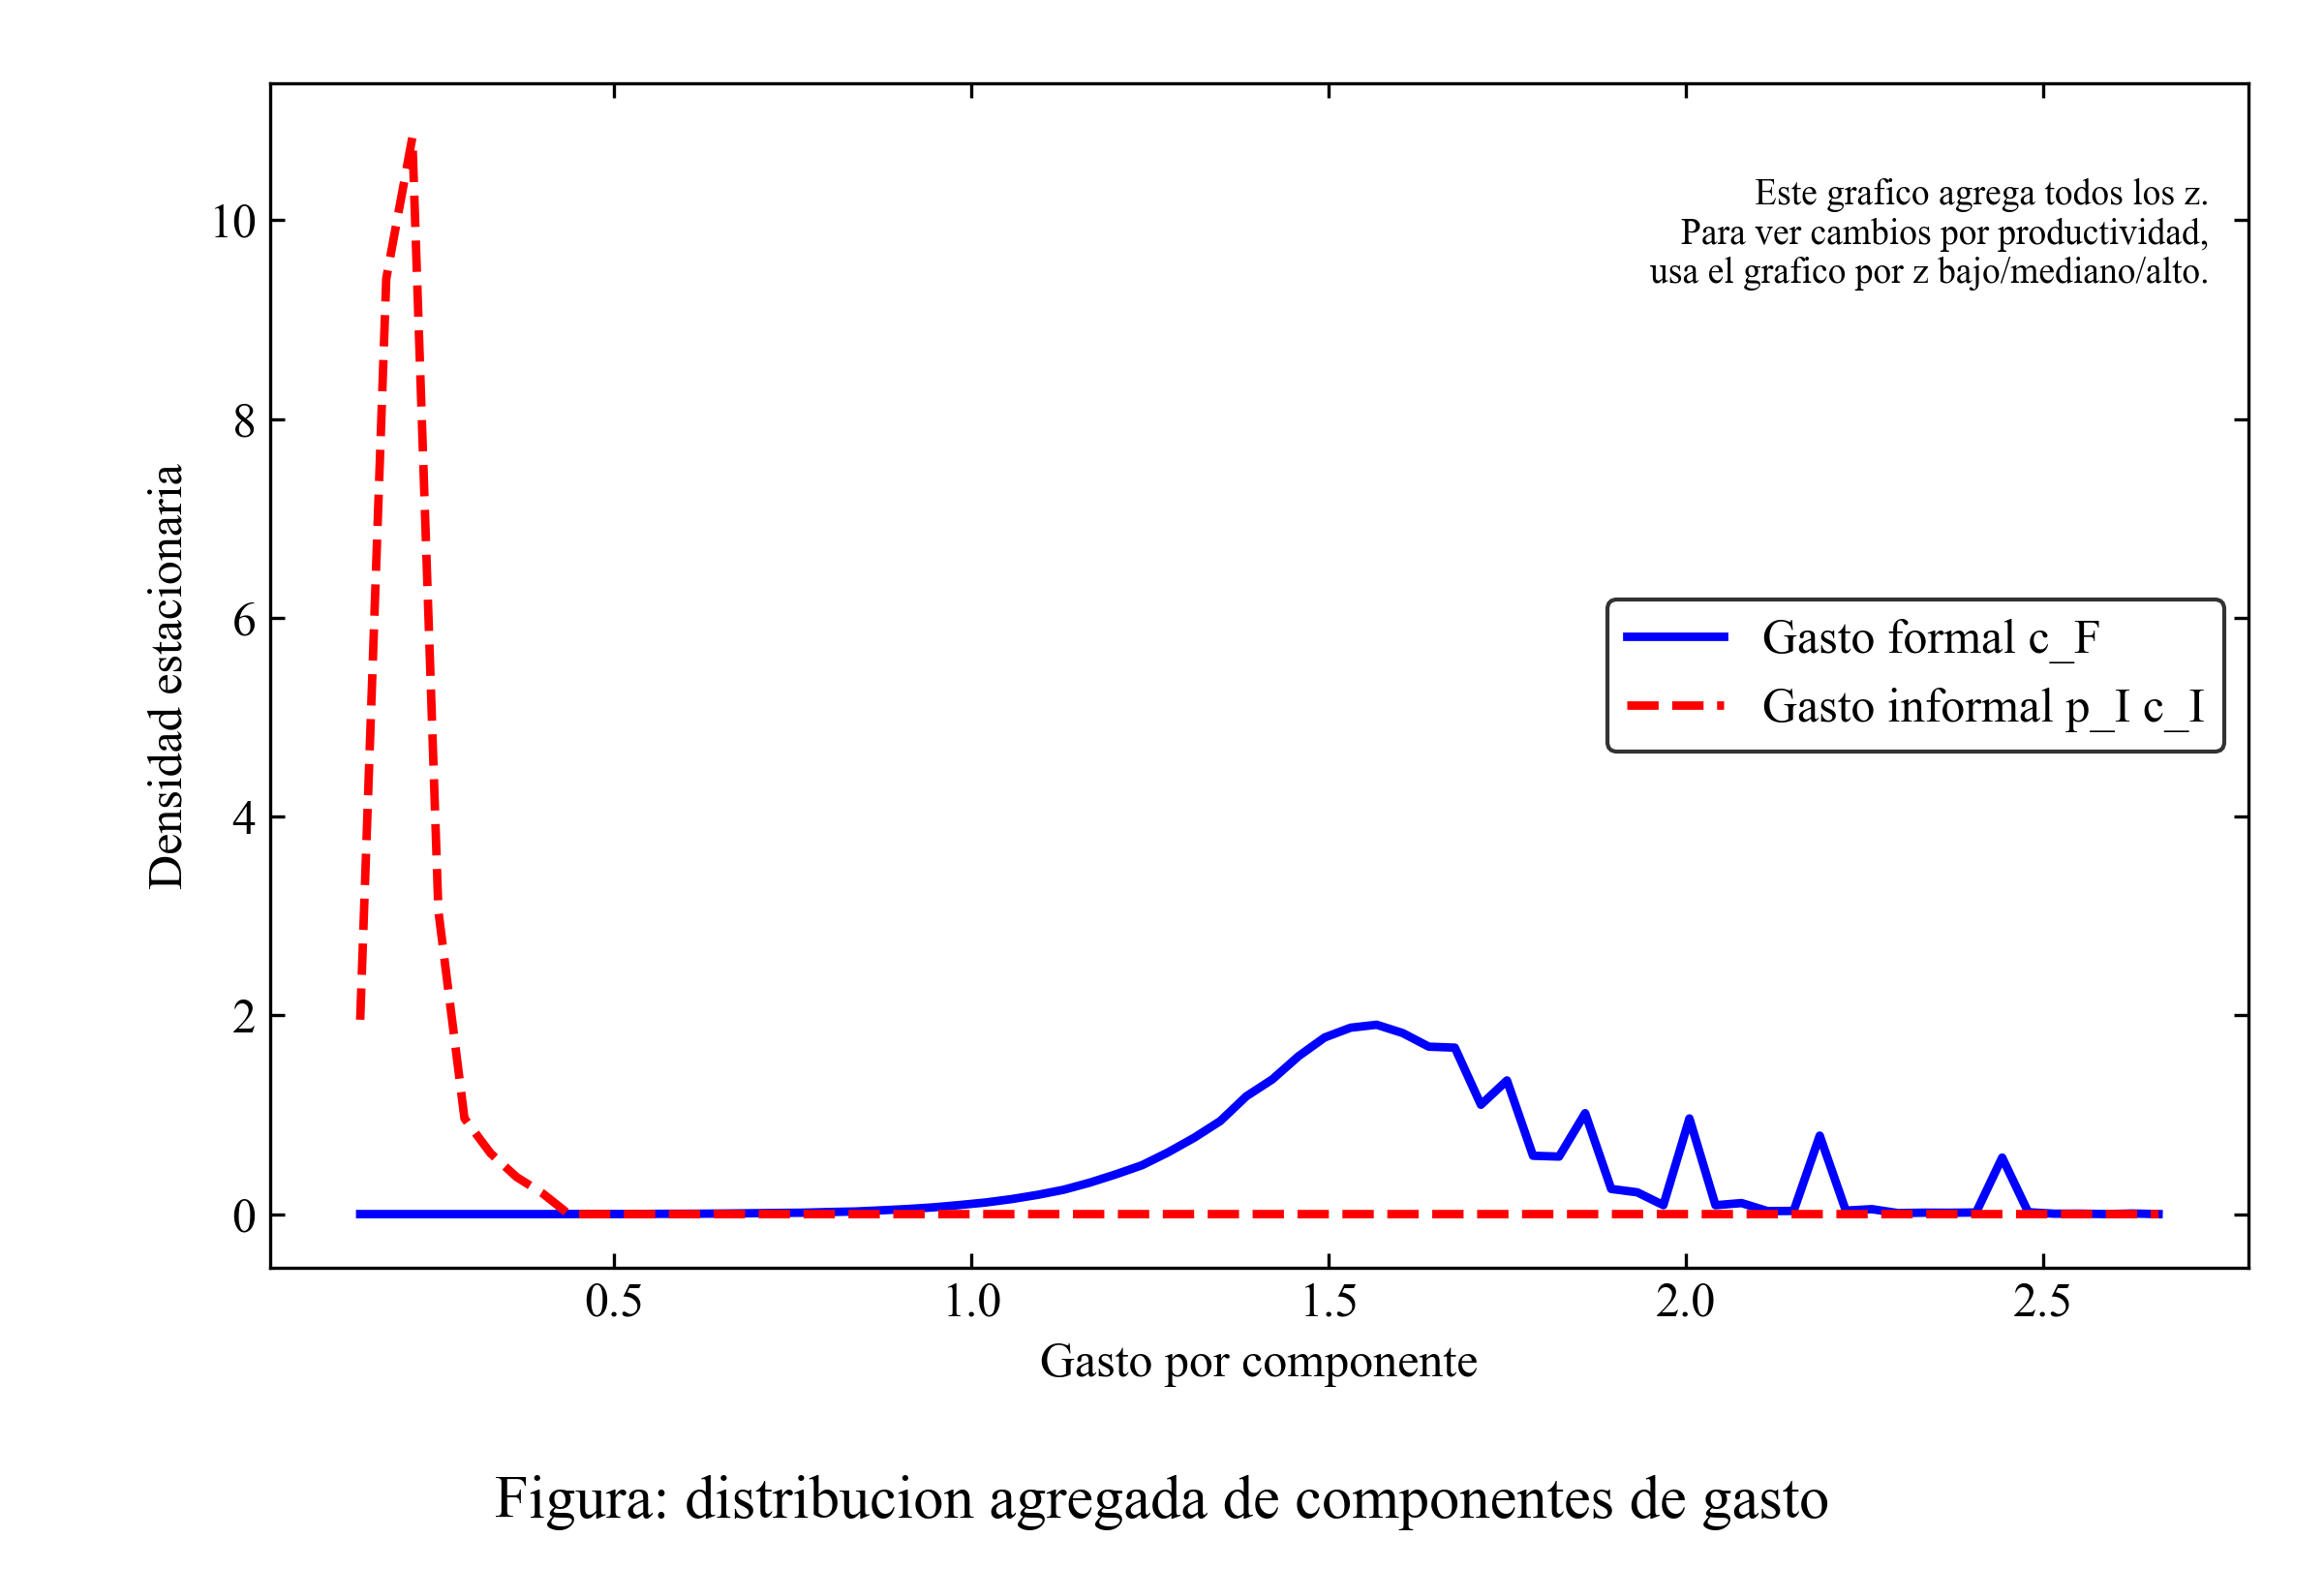
\includegraphics[width=0.94\textwidth,height=0.72\textheight,keepaspectratio]{moll_consumption_components_distribution.png}
  \vspace{0.1cm}

  \small
  La canasta CES separa consumo formal e informal y permite interpretar el gasto monetario total del hogar.
\end{frame}

\begin{frame}{Mensaje para la defensa}
  \begin{block}{Resultado central}
    El modelo reproduce el sorting por productividad (mayor $z$ $\rightarrow$ m\'as formalidad) y la trampa de baja acumulaci\'on: hogares de baja productividad dependen m\'as del sector informal y acumulan menos riqueza.
  \end{block}
  \vspace{0.2cm}
  \begin{block}{Calibraci\'on en curso}
    \small
    T4 (horas informales) clavado en 0.52--0.56. T5 (PBI informal) en 0.09--0.16, tensi\'on con $p_I{<}1$. Hong (2022) $\rho_z{=}0.86$ eleva ahorro precautorio $\rightarrow$ $w_F/w_I$ alto $\rightarrow$ T5 estructuralmente bajo. Pr\'oximo: $\omega_C{\approx}0.60$ con DRS G\"obel.
  \end{block}
  \vspace{0.2cm}
  \begin{block}{Limitaci\'on principal}
    Sin margen extensivo. T6 (gap informalidad por riqueza) $\approx 0.04$ vs dato 0.53. Requiere elecci\'on discreta formal/informal.
  \end{block}
\end{frame}

\begin{frame}{Calibraci\'on: targets vs modelo}
  \small
  \renewcommand{\arraystretch}{1.25}
  \begin{tabularx}{\textwidth}{>{\bfseries}p{0.22\textwidth} c c c X}
    \toprule
    Target & Modelo & Dato Per\'u & Brecha & Instrumento \\
    \midrule
    T4: $L_I/(L_F+L_I)$ & \textbf{0.520} & 0.557 & $-$0.037 & $\psi_F/\psi_I$ \\
    T5: $p_I Y_I / (Y_F + p_I Y_I)$ & \textbf{0.094} & 0.190 & $-$0.096 & $A_I$, $\omega_C$ \\
    Tkz: gap formal $z_2-z_1$ & \textbf{0.163} & 0.386 & $-$0.223 & $\kappa_{z1}$ \\
    Tgasto: $E[\text{gasto}\mid l_F>l_I]/E[\text{gasto}\mid l_I\geq l_F]$ & \textbf{1.34} & 1.91 & $-$0.57 & sorting \\
    \midrule
    \multicolumn{5}{l}{\footnotesize Referencia no calibrada:} \\
    T1: $w_F / (w_I\,\theta)$ hogar & \textbf{3.93} & $\sim$2.30 & $+$1.63 & — \\
    T6: gap informal $Q_1-Q_5$ & \textbf{0.04} & 0.53 & $-$0.49 & extensivo \\
    \bottomrule
  \end{tabularx}
  \vspace{0.25cm}
  \begin{block}{Estado}
    \footnotesize
    Hong (2022) $\rho_z{=}0.86$. DRS G\"obel $\alpha_I{=}0.118,\beta_I{=}0.605$. $\omega_C{=}0.65$, $\nu_I{=}0.40$. \textbf{$p_I{=}0.77$} \checkmark. T4 cerca. T5 y Tkz en progreso. Pr\'oximo: bajar $\omega_C$ a 0.60 para subir T5 manteniendo $p_I<1$.
  \end{block}
\end{frame}

\begin{frame}{Limitaciones actuales}
  \small
  \renewcommand{\arraystretch}{1.18}
  \begin{tabularx}{\textwidth}{>{\bfseries}p{0.30\textwidth} X}
    \toprule
    Dimensi\'on & Implicancia para los resultados \\
    \midrule
    Margen extensivo ausente & No hay elecci\'on discreta formal/informal; todos asignan horas a ambos sectores. Limitaci\'on central: explica bajo ajuste de T6 (0.04 vs 0.53). \\
    Tensi\'on estructural Hong & $\rho_z{=}0.86$ (Hong 2022) eleva ahorro precautorio $\rightarrow$ $w_F/w_I{\approx}4$ (dato BCR $\sim$2.3). T5 nominal m\'aximo alcanzable $\approx$0.15 con $p_I{<}1$. \\
    Mercado de impago ausente & Deuda entra como restricci\'on y prima ex\'ogena; sin default end\'ogeno. \\
    Sector informal agregado & Una sola tecnolog\'ia informal; se pierde heterogeneidad sectorial (agricultura, construcci\'on, comercio, servicios). \\
    Firmas sin decisi\'on & No hay entrada/salida de firmas ni elecci\'on de formalizaci\'on por parte de las empresas. \\
    \bottomrule
  \end{tabularx}
\end{frame}

\begin{frame}{Extensiones posibles}
  \scriptsize
  \begin{columns}[T,onlytextwidth]
    \begin{column}{0.50\textwidth}
      \textbf{Mercado laboral y formalizaci\'on}
      \begin{itemize}
        \item Costo de entrada end\'ogeno y elecci\'on ocupacional discreta \cite{achdou2017,mollcodes}.
        \item Barrera formal vinculada a capital humano, experiencia o b\'usqueda laboral \cite{mollcodes}.
        \item Transiciones tipo MIT shock para reformas tributarias, regulatorias o crediticias \cite{mollcodes}.
      \end{itemize}
    \end{column}
    \begin{column}{0.46\textwidth}
      \textbf{Heterogeneidad y fricciones}
      \begin{itemize}
        \item Default end\'ogeno y mercado de impago \cite{mollcodes}.
        \item M\'ultiples sectores informales y firmas heterog\'eneas \cite{mollcodes}.
        \item G\'enero, hogares de dos miembros y ciclo de vida \cite{bacher2025,mollcodes}.
        \item Validaci\'on externa: Colombia, M\'exico y Chile.
      \end{itemize}
    \end{column}
  \end{columns}
  \vspace{0.15cm}
  \begin{block}{Interpretaci\'on}
    La prioridad natural es pasar de informalidad intensiva a participaci\'on sectorial discreta: es la extensi\'on m\'as alineada con los targets que a\'un no se ajustan.
  \end{block}
\end{frame}

\begin{frame}[allowframebreaks]{Bibliograf\'ia}
  \footnotesize
  \begin{thebibliography}{9}
    \bibitem{achdou2017}
    Achdou, Y., Han, J., Lasry, J.-M., Lions, P.-L. y Moll, B. (2017).
    \newblock \emph{Income and Wealth Distribution in Macroeconomics: A Continuous-Time Approach}.
    \newblock Numerical appendix and HACT finite-difference methods.

    \bibitem{mollcodes}
    Moll, B. (2015--2026).
    \newblock \emph{Heterogeneous Agent Models in Continuous Time: Codes}.
    \newblock Incluye Huggett/Aiyagari, oferta laboral end\'ogena, MIT shocks, ciclo de vida, capital humano, activos l\'iquidos e il\'iquidos, firmas heterog\'eneas, default y matching laboral.
    \newblock \url{https://benjaminmoll.com/codes/}

    \bibitem{bacher2025}
    Bacher, A., Gr\"ubener, M. y Nord, L. (2025).
    \newblock Modelo de hogares de dos miembros, fricciones laborales y \emph{Added Worker Effect}.

    \bibitem{goenka2025}
    Goenka, A., Liu, L., Nguyen, T. y Pang, X. (2025).
    \newblock HACT con fricciones laborales y shocks clim\'aticos de productividad.
  \end{thebibliography}
\end{frame}

\end{document}
